\documentclass[a4paper]{article}
    \usepackage{fullpage}
    \usepackage{amsmath}
    \usepackage{amssymb}
	\usepackage{textcomp}
	\usepackage{graphicx}
	\usepackage[export]{adjustbox}
    \usepackage[utf8]{inputenc}
    \usepackage[T1]{fontenc}
    \usepackage[margin=1in]{geometry}
    \textheight=10in
    \pagestyle{empty}
    \raggedright

    %\renewcommand{\encodingdefault}{cg}
%\renewcommand{\rmdefault}{lgrcmr}

\def\bull{\vrule height 0.8ex width .7ex depth -.1ex }

% DEFINITIONS FOR RESUME %%%%%%%%%%%%%%%%%%%%%%%

\newcommand{\area} [2] {
    \vspace*{-9pt}
    \begin{verse}
        \textbf{#1}   #2
    \end{verse}
}

\newcommand{\lineunder} {
    \vspace*{-8pt} \\
    \hspace*{-18pt} \hrulefill \\
}

\newcommand{\header} [1] {
    {\hspace*{-18pt}\vspace*{6pt} \textsc{#1}}
    \vspace*{-6pt} \lineunder
}

\newcommand{\employer} [3] {
    { \textbf{#1} (#2)\\ \underline{\textbf{\emph{#3}}}\\  }
}

\newcommand{\contact} [3] {
    \vspace*{-10pt}
    \begin{center}
        {\Huge \scshape {#1}}\\
        #2 \\ #3
    \end{center}
    \vspace*{-8pt}
}

\newenvironment{achievements}{
    \begin{list}
        {$\bullet$}{\topsep 0pt \itemsep -2pt}}{\vspace*{4pt}
    \end{list}
}

\newcommand{\schoolwithcourses} [4] {
    \textbf{#1} #2 $\bullet$ #3\\
    #4 \\
    \vspace*{5pt}
}

\newcommand{\school} [4] {
    \textbf{#1} #2 $\bullet$ #3\\
    #4 \\
}
% END RESUME DEFINITIONS %%%%%%%%%%%%%%%%%%%%%%%

    \begin{document}
\vspace*{-40pt}

    

%==== Profile ====%
\vspace*{-10pt}
\begin{figure}[htp]
	\begin{minipage}{.3\textwidth}
		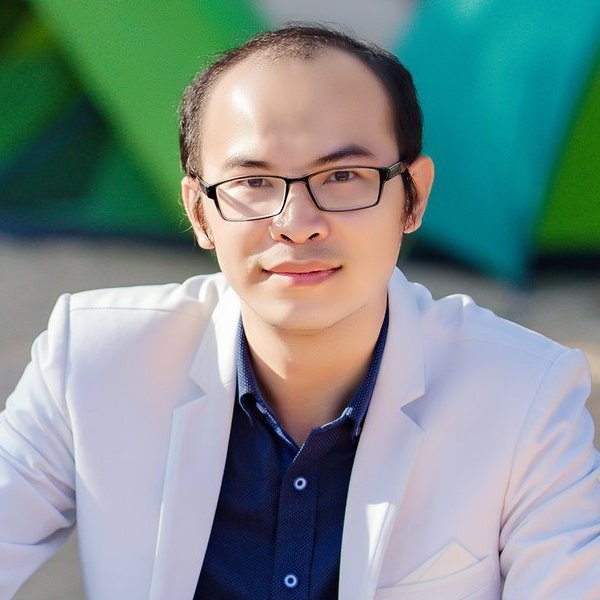
\includegraphics[width=3cm, frame=.2em]{Avatar.JPG}
	\end{minipage}
	\begin{minipage}{.7\textwidth}
		\begin{center}
			{\Huge \scshape {Nguyen Phu Phong}}\\
			"\textit{Experienced Software Engineer, passionating in changing the world with new technologies.}" \\
		\end{center}
	\end{minipage}
\end{figure}

%==== Personal Information ====%
\header{Personal Information}
\begin{tabular}{ l l }
	Fullname:                    & Nguyen Phu Phong \\
	Gender:                     & Male \\
	Academy Degrees: 			& Master's degrees (MBA \& MSE) \\
	Working Year's Experience: & 9 years \\
	Major: & Software Development \\
	Nationality:               & Vietnam \\
	Date of Birth:                       & 01 Aug 1988 \\
	Maritial Status:                     & Married                                              \\
	Contact Address:                    & 106/4F6, 11 Street, 11 Ward, Go Vap District, HCM City, Vietnam \\
	Cellphone:                         & +84 827 548 190 \\
	Email:			& nguyenphuphong@gmail.com \\
	Languages: & Vietnamese (Mother Language), English (Good)
\end{tabular}
\vspace{2mm}

%==== Education ====%
\header{Education}
\textbf{University of Bordeaux}\hfill Ho Chi MInh City, Vietnam\\
(MSc) Master of Software Engineering \hfill Sep 2017 - Oct 2019\\
\vspace{2mm}
\textbf{Open University Malaysia}\hfill Ho Chi Minh City, Vietnam\\
(MBA) Master of Business Administration \hfill Mar 2016 - Sep 2018\\
\vspace{2mm}
\textbf{University of Greenwich}\hfill Ho Chi Minh City, Vietnam\\
(BSc) Bachelor in Computer Science \hfill Jan 2010 - Feb 2011\\
\vspace{2mm}
\textbf{FPT Aptech}\hfill Ho Chi Minh City, Vietnam\\
Higher Diploma in Software Engineering \hfill Oct 2007 - Nov 2009\\
\vspace{2mm}

\header{Skills}
\begin{tabular}{ l l }
	Programming:                    & Java, Javascript, ReactJS, HTML, CSS, NodeJS, Bash                     \\
	Frameworks:                     & Spring, Struts, JSF, Selenium \\
	Operation System:               & Window, Linux(Ubuntu, CentOS)                                                \\
	Database:                       & Oracle, MySQL, PostgreQL, MongoDB                               \\
	Web Server:                     & Tomcat, WebLogic                                            \\
	Support Tools: 					& SVN, Git, Maven                                                     \\
	CI/CD:							& Jenkins, Team City \\
	Methodology:                    & Waterfall, Agile (Scrum, Kanban)                              \\
	Others:                         & AWS, Docker, Kubernetes                                       \\
\end{tabular}
\vspace{2mm}

%==== Certifications ====%
\header{Certifications}
\textbf{Developing on AWS}\hfill AWS Training\\
Certified Developing on AWS \hfill Oct 2019\\
\vspace{2mm}
\textbf{AWS Technical Essentials}\hfill AWS Training\\
Certified AWS Technical Essentials \hfill Oct 2019\\
\vspace{2mm}
\textbf{LeSS}\hfill LeSS\\
Certified LeSS Practitioner Designation \hfill Dec 2018\\
\vspace{2mm}
\textbf{ITIL Foundation}\hfill Apex Global Corporation\\
Certified of Completion ITIL Foundation \hfill Dec 2018\\
\vspace{2mm}
\textbf{Agile Certified Professonal}\hfill ICAgile\\
The International Consortium for Agile (ICAgile) \hfill Sep 2018\\
\vspace{2mm}
\textbf{HIPPA}\hfill HIPPATraining.com\\
HIPPA Awareness for Business Associates \hfill Apr 2017\\
\vspace{2mm}
\textbf{TOIEC}\hfill IIG\\
745 out of 990 (Listening: 415, Reading: 330) \hfill Feb 2016\\
\vspace{2mm}

\newpage

%==== Experience ====%
\header{Experience}
\vspace{1mm}

\textbf{Commonwealth Bank - Tyme Bank} \hfill Ho Chi Minh City, Vietnam\\
\textit{Senior Software Engineer/Back-End API Developer} \hfill Apr 2018 | Present\\
\vspace{-1mm}
\begin{itemize} \itemsep 1pt
	\item In a team to build up Back-End microserices banking systems
	\item Solving complex technical and business problems and learn new technology and frameworks.
	\item Driving best practice cyber security solutions and remaining on the forefront of emerging industry practices.
	\item Provides technical direction for the development, design, and systems integration for client engagement from definition phase through implementation.
	\item Custodian of Development Best practices, Development Technology direction/roadmap and application.
	\item Provides technical direction for the development, design, and systems integration for client engagement from definition phase through implementation.
	\item Facilitate team and other stakeholders meetings and deliver engaging, informative, well-organized presentations.
\end{itemize}
\textbf{KMS Technology, Inc.} \hfill Ho Chi Minh City, Vietnam\\
\textit{Senior Software Engineer/Team Leader} \hfill Apr 2017 | Mar 2018\\
\vspace{-1mm}
\begin{itemize} \itemsep 1pt
	\item Can be assigned to play the role of software architect, project lead, technical lead, or developer in a project
	\item Select the most appropriate technical solution and demonstrate the proposed solution to the client and the development team
	\item Design, document and implement the software architecture which addresses both functional and non-functional requirements such as performance, scalability, security, extensibility, and reliability etc
	\item Design/implement or supervise the implementation of the system and subsystems
	\item Mentor and provide guidance to other developers in the team
	\item Lead or participate in code review sessions
\end{itemize}
\textbf{ELCA Information Technology, Vietnam} \hfill Ho Chi Minh City, Vietnam\\
\textit{Senior Software Engineer/Fullstack Developer} \hfill Aug 2015 | Mar 2017\\
\vspace{-1mm}
\begin{itemize} \itemsep 1pt
	\item Develop mission-critical distributed applications for a broad range of clients and industries, using state-of-the-art tools and agile methodologies.
	\item Work closely with business analysts and software architects to design reliable, secure and highly efficient systems; participate directly in technical decisions.
	\item Be actively involved in the complete project lifecycle, from requirements analysis to final delivery.
	\item Contribute to knowledge sharing and continuous improvement activities.
\end{itemize}
\textbf{NTT Data Vietnam} \hfill Ho Chi Minh City, Vietnam\\
\textit{Senior Software Engineer/System Analyst} \hfill Dec 2014 | Jul 2015\\
\vspace{-1mm}
\begin{itemize} \itemsep 1pt
	\item Translates requirements defined by business analyst into logical, economical and practical system designs.
	\item Analyzes and Designs system flow and procedures to ensure optimum control and security of data and efficient use of resources.
	\item Prepares detailed specifications from which complete sets of programs will be written.
	\item Perform the role of Quality Assurance when system is ready.
	\item Support System installation, User training \& system maintenance
\end{itemize}

\newpage

\textbf{NTT Data Vietnam} \hfill Ho Chi Minh City, Vietnam\\
\textit{Software Engineer/Software Developer} \hfill Apr 2011 | Dec 2014\\
\vspace{-1mm}
\begin{itemize} \itemsep 1pt
	\item Responsible for the development of major components or modules and contribute to the design and maintenance of the products.
	\item Create quality source code, document code and procedures thoroughly as prescribed by the engineering standards.
	\item Use common development tools such as compilers, debuggers, profiling tools and source control system as prescribed by the engineering standards.
	\item Read \& understand design specifications, implement \& test software components (unit testing)
\end{itemize}

\header{Projects}
\begin{center}
	\textbf{\textit{Products}}
\end{center}

{\textbf{Tyme Digital Bank}} {\sl Spring Cloud, AWS, Kubernetes} \hfill https://www.tymebank.co.za/\\
TymeBank is a new kind of bank that’s digitally smart. The money we save by not having branches benefits you, it means you pay a lot less for banking. We have no monthly fees, many everyday banking transactions are FREE and there are very low charges for other transactions.\\
\vspace*{2mm}
{\textbf{HotSchedules}} {\sl NodeJS, Mongo, AWS} \hfill https://www.hotschedules.com/\\
A restaurant management plaform which build on cloud.\\
\vspace*{2mm}
{\textbf{Event Management Tools}} {\sl Java, Spring Core, Spring Batch, JSF, Oracle} \hfill https://www.elca.ch/en/news/2018/credit-suisse-individual-solution-was-more-cost-effective\\
A tool to manage event at Credit Suisse Bank\\
\vspace*{2mm}

\begin{center}
	\textbf{\textit{Offshore \& Outsourcing}}
\end{center}

{\textbf{Informatica}} {\sl Java, Struts, Bash}\\
Cloning and Transform Data from Banking Source, support to expose testing data which don't violate confidential information.\\
\vspace*{2mm}
{\textbf{MOTAS}} {\sl Java, Struts, HTML, CSS}\\
Myanmar Vehicle Registration System\\
\vspace*{2mm}
{\textbf{Currency Exchange System}} {\sl Java, Struts, HTML, JQuery}\\
Myanmar Vehicle Registration System\\
\vspace*{2mm}
{\textbf{TARBAL}} {\sl Java, Selenium, Open2Test}\\
Automation test for financial system\\
\vspace*{2mm}
{\textbf{MyLink}} {\sl Java, Spring, Struts, iBatis, SOAP Services}\\
Automation test for financial system\\
\vspace*{2mm}
{\textbf{R\&D}} {\sl Hadoop, Pig, Hive}\\
Building a Big Data system based on Hadoop.\\
\vspace*{2mm}

\header{Reference Contacts:}
\textbf{Huynh Duc Tin}\hfill Project Manager\\
NTT Data Vietnam \hfill %0779 448 579% \\
\vspace{2mm}

\textbf{Quang Trong An}\hfill Project Manager\\
ELCA Co. Ltd \hfill %0909 572 110%\\
\vspace{2mm}

\textbf{Ngo Thanh Hai}\hfill Team Leader\\
KMS Vietnam \hfill %0973 433 168%\\
\vspace{2mm}

\textbf{Nguyen Hoang Quan}\hfill Solution Delivery Manager\\
CBA/TYME Digital \hfill %0913 968 985%\\
\vspace{2mm}

\end{document}
